\documentclass[a4paper,12pt]{report}
\usepackage[utf8]{inputenc}
\usepackage[spanish]{babel}  % Cambia el idioma a español
\usepackage{geometry}
\usepackage{setspace}
\usepackage{titlesec}
\usepackage{graphicx}
\usepackage{hyperref} % Paquete para enlaces clicables
\usepackage{placeins} % per a les float barrier, que no es moguin les imatges.
\usepackage{titlesec}  % Paquete para personalizar títulos
\usepackage{float}  %pquete para que las figuras no se de splacen
\usepackage{listings} %para poner entronos de codigo 

% Configuración para reducir el espacio superior de los capítulos
\titleformat{\chapter}[hang]
{\normalfont\huge\bfseries} % Formato de la fuente y tamaño del capítulo
{Capítulo \thechapter}{0pt}{\huge}  % Sin espacio entre "Capítulo X" y el título
\titlespacing*{\chapter}{0pt}{-20pt}{20pt} % Ajustes de espacio antes, después, y debajo del título




\usepackage{xcolor} % Para definir colores personalizados

% Configuración del estilo para Git
\lstset{
	language=bash,                   % Usa Bash para sintaxis similar a Git
	basicstyle=\ttfamily\small,      % Texto monoespaciado y pequeño
	keywordstyle=\bfseries,          % Palabras clave en negrita
	commentstyle=\color{gray},       % Comentarios en gris
	morekeywords={git, clone, add, branch, checkout, commit, push}, % Palabras clave de Git
	showstringspaces=false           % No mostrar espacios en cadenas de texto
}



% Configuración de márgenes
\geometry{left=3cm, right=3cm, top=2.5cm, bottom=2.5cm}

% Configuración de espacios
\setstretch{1.15}


% Configuración de formato de títulos
\titleformat{\chapter}[display]
{\normalfont\bfseries\Huge}
{}{0pt}{\Huge}

\hypersetup{
	colorlinks=true,        % Colorear enlaces
	linkcolor=blue,         % Color de los enlaces internos
	urlcolor=blue,          % Color de los enlaces externos (URLs)
	pdftitle={Memoria Proyecto}, % Título del PDF
	pdfauthor={Jorge Muñoz Carrión, Santiago Sánchez Sans} % Autor
}

\begin{document}
	
	

	
	
	
	% Portada
	\begin{titlepage}
		\begin{center}

			
			\vspace*{5cm} 

			\LARGE{Creación de un dashboard para usuarios del ticket digital de Mercadona: que permita consultara evolución de productos habitualmente adquiridos, el coste de sus compras por períodos temporales y el monto de gastos por áreas de producto}
			
			\vfill
			
		\begin{flushright}
			\large{\textbf{Santiago Sánchez Sans}}
			
			\large{\textit{Ciclo formativo en desarrollo de aplicaciones web}}
			
			\large{Memoria del Proyecto de DAW}
			
			\large{IES Abastos. Curso 2024/25. Grupo 7X. XX de Junio de 2025}
			
			\large{Tutor Individual: Carlos Furones}
		\end{flushright}

			
			
			% Fecha
			
			
		\end{center}
	\end{titlepage}
	
	% Índice
	\tableofcontents
	\newpage
	
	
	
	
	
	
	
	
	% Per a conseguir que els espais apliquin solsament a les seccions no a l'index
	\begingroup
	\setlength{\parskip}{.7em}
	
	
	% Capítulos y secciones
	\chapter{Introducción}

		\section{¿Qué es el ticket digital de Mercadona?}
		
		Mercadona implementa un sistema de tickets digitales que vinculan la tarjeta de débito a un correo electrónico. Cualquier usuario del supermercado que quiera utilizar el ticket digital solamente deberá facilitar estos dos datos y el supermercado le enviará por correo electrónico los tickets de las posteriores compras hechas en cualquier establecimiento de Mercadona.
		
		Las ventajas para el usuario son evidentes: no se pierden los tickets de cara a devoluciones y el cliente del supermercado no debe esperar a la impresión del ticket.
		
		
		
		\section{Identificación de necesidades}
		\label{section:identificacionNecesidades}
		
		Los tickets de cada usuario se acumulan de forma recurrente en el correo electrónico y con un formato estructurado (los asuntos son predecibles e incluyen las fechas) y dentro de cada correo de un ticket digital se encuentra un PDF con el desglose de la compra (producto, unidades vendidas, establecimiento, etc).
		
		Esta información se acumula en el correo del usuario pero a pesar de ser una información estructurada su acceso para el usuario no es simple: no puede visualizar lo que ha gastado, ni el precio de los productos y de su evolución, ni los supermercados en los que ha comprado, ni las veces que lo ha hecho, etc.

		\section{Objetivos del proyecto} % OBLIGAT
		\label{section:objetivosProyecto}
		
		Este proyecto quiere responder a estas necesidades. Para ello se plantea la Creación de un dashboard o "cuadro de mando" front-end para que un usuario del ticket digital de Mercadona pueda visualizar la evolución de precios de los productos adquiridos, el coste promedio de sus compras por períodos temporales y sus distribuciones de gastos a partir de los tickets digitales guardados en una base de datos.
		
		
		Los \textbf{Objetivos principales} del proyecto son mostrar al usuario:

					
		\begin{itemize}
			\setlength{\itemsep}{-.5em}
			\item \textbf{Evolución de precios} (inflación) a lo largo del tiempo en los productos habitualmente comprados en el mismo establecimiento\footnote{La evolución de precios se mostrará solamente para un mismo centro de Mercadona, dado que distintos centros pueden cambiar los nombres de los productos (por ejemplo, en Cataluña…).}.
			\item \textbf{Evolución del gasto} total del usuario a lo largo del tiempo.
		\end{itemize}
		
		
		

		
		

		
		
		
		
		
		
		
		
		
		
			%IDENTIFICAR OBJECTIUS  %OBLIGAT
			%JUSTIFICAR OBJECTIUS   %OBLIGAT
			
			
	
		
	

		



		
	

		
	

		


		
		%imagen barra navegación nuestra (emulando accenture)
		\setlength{\belowcaptionskip}{10pt}
		\FloatBarrier
		\begin{figure}[H]
			\centering
			\caption{nuestra ``NavBar": fondo negro, letra blanca y un solo desplegable.}
			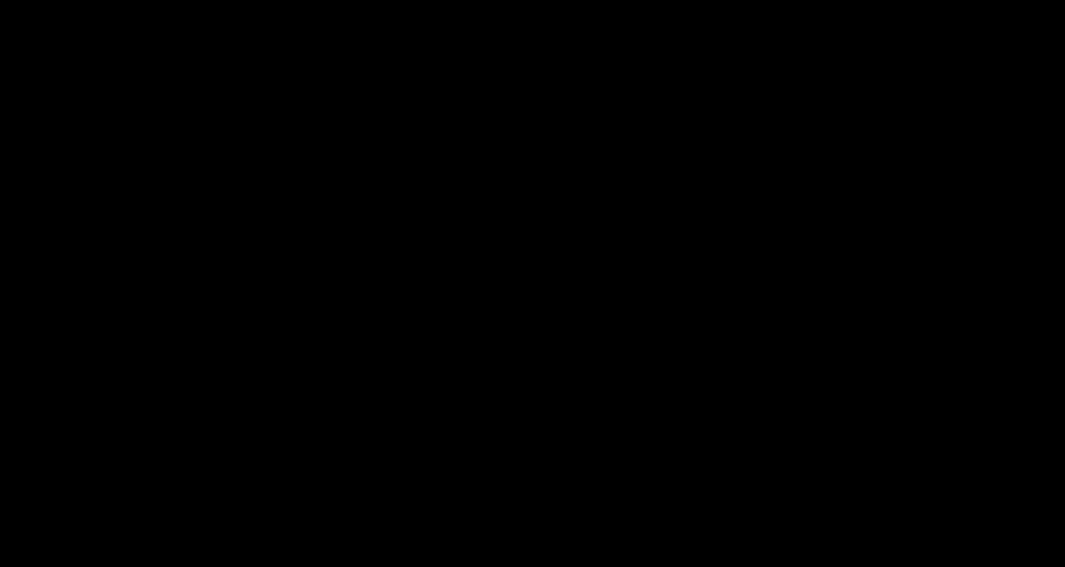
\includegraphics[width=1\textwidth]{img/sampleta.png}
			\label{fig:etiquetaNavBarNuestra} 
		\end{figure}
		\FloatBarrier
		
		
		
		
	
	\chapter{Diseño del proyecto}  %OBLIGAT
	
		
				
		Para implementar los objetivos principales de los que hemos hablado en la sección \ref{section:objetivosProyecto} hemos proyectado una serie de requisitos funcionales de la aplicación.
		
		


		
		
		
		
		\section{Requisitos Funcionales}
		
			\subsection{Requisitos de la aplicación}
			
			
			\textbf{REQUISITO A:} Mostrar evolución de los precios de los productos unitarios adquiridos con más frecuencia (visualizable en un gráfico donde en X tendremos el tiempo y en Y el precio en euros). Para los productos de precios muy variables (productos a granel, como frutas, etc.), se mostrará la evolución del precio por kg a lo largo del tiempo.
			
			\textbf{REQUISITO B:} Coste total de la cesta de la compra del usuario a lo largo de distintas ventanas temporales (por meses, períodos de 3, 6 meses y un año), independientemente del centro de Mercadona en el que se compre (todos juntos).
			
			\textbf{REQUISITO C:} Al lado de este mismo coste total mostrado en B), se incluirá un diagrama de queso (o de sectores) desglosando qué porcentaje del dinero se ha destinado a cada una de las siguientes categorías: verdura y hortalizas, frutas, huevos y lácteos, agua y bebidas, aceite y especias, carnes, pescado, hogar e higiene personal.
			Para ello, dado que no tenemos categorizados todos los productos de Mercadona ni podríamos hacerlo por falta de una lista exhaustiva y de tiempo, se usará un modelo predictivo con word embeddings (módulo Spacy) y cosine similarity (sklearn) para encontrar distancias pequeñas entre las descripciones de los tickets y las categorías, facilitando así la clasificación.
			
			
			
			\textbf{REQUISITO D:} Un botón ``Actualizar'' permitirá al usuario refrescar los datos desde el servidor cuando haya añadido nuevas compras. También podríamos permitir que los PDFs descargados en el servidor se almacenen en una carpeta local del usuario para que pueda verificar la extracción de los datos.
			
			\textbf{REQUISITO E:} Hacer un sistema front-end y back-end que permitan redirigir a los usuarios rápidamente a un registro de forma inteligente. Nos inspiraremos en el sistema de registro e iniciar sesión de NetFlix \textbf{(POSAR DIAGRAMA A L'ANEX SOBRE EL SISTEMA DEL NETFLIX I EL NOSTRE)}
			
			\subsection{Requisitos de los usuarios}
			
			El correo electrónico y la contraseña de la cuenta de Gmail de alguien que sea usuario del ticket digital de Mercadona y tenga decenas de tickets digitales por analizar, con compras estables y productos recurrentes.
			
			Nota: En la demo se proporcionarán ya muchos tickets digitales (tickets míos, que cederé para mostrar la utilidad de la aplicación). No será necesario recurrir a la extracción de datos de otro usuario de ticket digital. Se mostrarán un mínimo de tickets digitales en un mismo centro de Mercadona para poder evidenciar la evolución de precios y gastos.
			
		
		\section{Stack tecnológico}
	
		Hemos escogido un stack tecnológico que permite que seamos fieles a los requisitos funcionales que nos hemos marcado para la aplicación:
		
			 \subsection{Front-End: HTML, CSS y Javascript}
			 
			Se ha usado HTML, CSS y JavaScript. - Para la visualización de gráficos se usará una librerría javascript: https://www.chartjs.org/. Entre otras cosas se utilizará para hacer los gráficos de la evolución de precios por producto.
			
	
		 
		\subsection{back-end: Java (SpringBoot) y Python}
		
			- Back-end con Java (springboot para el login y la autenticación de usuarios: con este framework guardaremos datos en la BBDD mySQL).
			
			- Python dentro de un contenedor docker (o python a secas, para descargar los pdfs del correo) y parsear el contenido de los mismos: con sklearn, numpy y spacy que luego se podrán pasarlos a la BBDD mongoDB.
			
		\subsection{BBDD: MySQL y MongoDB}
		
		
		Para guardar los datos de los usuarios se debe usar un sistema de gestión de base de datos relacional. Hemos escogido MySQL dado que es el que hemos visto en el grado superior y estamos bien versados en ello.
		
		Sin embargo, los productos de Mercadona no los conocemos de antemano ni tenemos una lista exhaustiva de los mismos. Además, el número de productos que se pueden encontrar en un ticket varía en cada compra, por lo que no podemos usar una base de datos relacional tradicional como MySQL o PostgreSQL por que se trata de información no estructurada. En su lugar, usaremos MongoDB, una BBDD NoSQL que almacena datos en formato JSON y permite, además, búsquedas eficientes.
		
		Para optimizar el backend, intentaremos que un usuario pueda consultar repetidamente sus compras sin sobrecargar el servidor. La primera vez que consulte sus datos, estos se descargarán y almacenarán en localStorage del cliente. En consultas posteriores, los datos se obtendrán directamente de localStorage sin necesidad de hacer peticiones al servidor. Evaluaremos la viabilidad de este sistema durante el desarrollo; Esto es la fase de diseño y como tal, \textbf{PUEDE QUE EN LA FASE DE DESARROLLO CAMBIE}, en caso de no ser factible, las consultas se harán directamente en MongoDB.
		



		
		
		
		
		
		\section{Diagramas de la aplicación}
		
		\textbf{Fer un diagrama guapo de tots els components de l'aplicació.}
	
	\chapter{Desarrollo del proyecto} %OBLIGAT
	

	
	
				
			\section{GitHub del proyecto}
			
				Para desarrollar este proyecto se ha trabajado con GitHub y git. Dado que no ha habido trabajo en equipo no se han utilizado pull requests a la rama main sino simplemente se ha seguido la estrategia de crear ramas de característica y, una vez son satisfactorias, hacer un merge en la rama main en local.
				
				Un flujo de trabajo habitual es mediante ramas de característica (puede verse anexo \ref{sec:anexoFlujoGit}). También puede verse el GitHub del proyecto a continuación. Dentro del readme del proyecto encontraréis instrucciones para su descarga, clonado y ``despliegue'' de sus componentes en vuestro ordenador personal si así lo deseáis.
			

			
			
			
			
			
			
			
			
			
			
			
			
			\begin{table}[h!]
				\centering
				\begin{tabular}{|p{3.8cm}|p{11cm}|}
					\hline
					\textbf{Link al repositorio} & \href{https://github.com/blackcub3s/mercApp}{https://github.com/blackcub3s/mercApp} \\
					\hline
					\textbf{Página desplegada} & TO DO \\ % Corregido: Se eliminó la llave extra
					\hline
				\end{tabular}
				\caption{Enlaces importantes del proyecto.}
				\label{tabla:enlaces}
			\end{table}

	
	
		
			\section{Entornos de desarrollo}
			
				Para el back-end de Java con SpringBoot se ha utilizado el editor Java \texttt{IntelliJ Idea community edition} que expone el backend en el puerto\textbf{ 8080}: se han utilizado extensiones necesarias para correr el proyecto que permiten sacar provecho de LomBok sin las cuales correr el proyecto en IntelliJ fallará.
				
				Para el frontend se ha utilizado \texttt{VScode}, con la extensión live server para poder hacer llamadas al back-end directamente desde el puerto \textbf{5500}. Esto podría hacer las veces de una CDN donde podrían estar alojados los archivos estáticos (HTML, CSS y JavaScript).
		
	
		
			\section{desarrollo del front-end}
		
			\section{desarrollo back-end}
	
	\chapter{Evaluación y Conclusiones Finales} %OBLIGAT
	

	
	
	
	

	
	
	\chapter{ANEXO}
	\label{chap:anexoFigma} % Esta es la etiqueta de referencia
		
			
			
			
		\section{Flujo de trabajo habitual en git}
		\label{sec:anexoFlujoGit}
		
\begin{lstlisting}[language=bash, basicstyle=\ttfamily\small]
	


# trabajamos con el proyecto y se introduce
# en el staging area
git add -A 

# creamos rama para aglutinar los cambios
git branch backEnd

# cambiamos a la rama que acabamos de crear
git checkout backEnd

# guardamos los cambios como nodos dentro de
# la rama con la que desarrollamos.	
git commit -m "commit 1"  	
git commit -m "commit 2"
# [...]
git commit -m "commit n"

#cambiamos a rama main local y luego integramos cambios
git checkout main
git merge backEnd

#Subimos los cambios al repo remoto
git push origin main 

	
\end{lstlisting}
		
	
	
		\section{CODIGO 2}
		\label{sec:ASDASDSA}

	
		\section{CODIGO 3}
		\label{sec:IJIIJIJ}
	

	
		\section{CODIGO 4}
		\label{sec:QWQOIR}
	

	
		\section{CODIGO 5}
		\label{sec:KLNASQOW}
	

		


		
	% Bibliografía (\chapter(6. Bibliograifa) como implicito)
	\addcontentsline{toc}{chapter}{7. Bibliografía} 
	\bibliographystyle{plain}  % Estilo de bibliografía
	\bibliography{referencias} % Nombre del archivo .bib  extensión
	
		
	

	\endgroup
\end{document}
